\documentclass[twoside]{book}

% Packages required by doxygen
\usepackage{calc}
\usepackage{doxygen}
\usepackage{graphicx}
\usepackage[utf8]{inputenc}
\usepackage{makeidx}
\usepackage{multicol}
\usepackage{multirow}
\usepackage{textcomp}
\usepackage[table]{xcolor}

% Font selection
\usepackage[T1]{fontenc}
\usepackage{mathptmx}
\usepackage[scaled=.90]{helvet}
\usepackage{courier}
\usepackage{amssymb}
\usepackage{sectsty}
\renewcommand{\familydefault}{\sfdefault}
\allsectionsfont{%
  \fontseries{bc}\selectfont%
  \color{darkgray}%
}
\renewcommand{\DoxyLabelFont}{%
  \fontseries{bc}\selectfont%
  \color{darkgray}%
}

% Page & text layout
\usepackage{geometry}
\geometry{%
  a4paper,%
  top=2.5cm,%
  bottom=2.5cm,%
  left=2.5cm,%
  right=2.5cm%
}
\tolerance=750
\hfuzz=15pt
\hbadness=750
\setlength{\emergencystretch}{15pt}
\setlength{\parindent}{0cm}
\setlength{\parskip}{0.2cm}
\makeatletter
\renewcommand{\paragraph}{%
  \@startsection{paragraph}{4}{0ex}{-1.0ex}{1.0ex}{%
    \normalfont\normalsize\bfseries\SS@parafont%
  }%
}
\renewcommand{\subparagraph}{%
  \@startsection{subparagraph}{5}{0ex}{-1.0ex}{1.0ex}{%
    \normalfont\normalsize\bfseries\SS@subparafont%
  }%
}
\makeatother

% Headers & footers
\usepackage{fancyhdr}
\pagestyle{fancyplain}
\fancyhead[LE]{\fancyplain{}{\bfseries\thepage}}
\fancyhead[CE]{\fancyplain{}{}}
\fancyhead[RE]{\fancyplain{}{\bfseries\leftmark}}
\fancyhead[LO]{\fancyplain{}{\bfseries\rightmark}}
\fancyhead[CO]{\fancyplain{}{}}
\fancyhead[RO]{\fancyplain{}{\bfseries\thepage}}
\fancyfoot[LE]{\fancyplain{}{}}
\fancyfoot[CE]{\fancyplain{}{}}
\fancyfoot[RE]{\fancyplain{}{\bfseries\scriptsize Generated on Tue Nov 26 2013 19\-:04\-:17 for Simple\-Lion -\/ P\-H\-P module by Doxygen }}
\fancyfoot[LO]{\fancyplain{}{\bfseries\scriptsize Generated on Tue Nov 26 2013 19\-:04\-:17 for Simple\-Lion -\/ P\-H\-P module by Doxygen }}
\fancyfoot[CO]{\fancyplain{}{}}
\fancyfoot[RO]{\fancyplain{}{}}
\renewcommand{\footrulewidth}{0.4pt}
\renewcommand{\chaptermark}[1]{%
  \markboth{#1}{}%
}
\renewcommand{\sectionmark}[1]{%
  \markright{\thesection\ #1}%
}

% Indices & bibliography
\usepackage{natbib}
\usepackage[titles]{tocloft}
\setcounter{tocdepth}{3}
\setcounter{secnumdepth}{5}
\makeindex

% Hyperlinks (required, but should be loaded last)
\usepackage{ifpdf}
\ifpdf
  \usepackage[pdftex,pagebackref=true]{hyperref}
\else
  \usepackage[ps2pdf,pagebackref=true]{hyperref}
\fi
\hypersetup{%
  colorlinks=true,%
  linkcolor=blue,%
  citecolor=blue,%
  unicode%
}

% Custom commands
\newcommand{\clearemptydoublepage}{%
  \newpage{\pagestyle{empty}\cleardoublepage}%
}


%===== C O N T E N T S =====

\begin{document}

% Titlepage & ToC
\hypersetup{pageanchor=false}
\pagenumbering{roman}
\begin{titlepage}
\vspace*{7cm}
\begin{center}%
{\Large Simple\-Lion -\/ P\-H\-P module \\[1ex]\large 0.\-1 }\\
\vspace*{1cm}
{\large Generated by Doxygen 1.8.5}\\
\vspace*{0.5cm}
{\small Tue Nov 26 2013 19:04:17}\\
\end{center}
\end{titlepage}
\clearemptydoublepage
\tableofcontents
\clearemptydoublepage
\pagenumbering{arabic}
\hypersetup{pageanchor=true}

%--- Begin generated contents ---
\chapter{Namespace Index}
\section{Namespace List}
Here is a list of all documented namespaces with brief descriptions\-:\begin{DoxyCompactList}
\item\contentsline{section}{\hyperlink{namespace_simple_lion}{Simple\-Lion} \\*A global namespace for the \hyperlink{namespace_simple_lion}{Simple\-Lion} project -\/ P\-H\-P module }{\pageref{namespace_simple_lion}}{}
\end{DoxyCompactList}

\chapter{Hierarchical Index}
\section{Class Hierarchy}
This inheritance list is sorted roughly, but not completely, alphabetically\-:\begin{DoxyCompactList}
\item Exception\begin{DoxyCompactList}
\item \contentsline{section}{File\-Exception}{\pageref{class_simple_lion_1_1_file_exception}}{}
\item \contentsline{section}{Filesystem\-Exception}{\pageref{class_simple_lion_1_1_filesystem_exception}}{}
\end{DoxyCompactList}
\item \contentsline{section}{Localization}{\pageref{class_simple_lion_1_1_localization}}{}
\item \contentsline{section}{Localization\-Category}{\pageref{class_simple_lion_1_1_localization_category}}{}
\item \contentsline{section}{Localization\-String}{\pageref{class_simple_lion_1_1_localization_string}}{}
\end{DoxyCompactList}

\chapter{Data Structure Index}
\section{Data Structures}
Here are the data structures with brief descriptions\-:\begin{DoxyCompactList}
\item\contentsline{section}{\hyperlink{class_simple_lion_1_1_file_exception}{File\-Exception} \\*An exception to be thrown on file error }{\pageref{class_simple_lion_1_1_file_exception}}{}
\item\contentsline{section}{\hyperlink{class_simple_lion_1_1_filesystem_exception}{Filesystem\-Exception} \\*An exception to be thrown on directory error }{\pageref{class_simple_lion_1_1_filesystem_exception}}{}
\item\contentsline{section}{\hyperlink{class_simple_lion_1_1_localization}{Localization} \\*A class representing the \hyperlink{class_simple_lion_1_1_localization}{Localization} engine }{\pageref{class_simple_lion_1_1_localization}}{}
\item\contentsline{section}{\hyperlink{class_simple_lion_1_1_localization_category}{Localization\-Category} \\*A class that represents category grouping localization strings }{\pageref{class_simple_lion_1_1_localization_category}}{}
\item\contentsline{section}{\hyperlink{class_simple_lion_1_1_localization_string}{Localization\-String} \\*A class representing a localized string }{\pageref{class_simple_lion_1_1_localization_string}}{}
\end{DoxyCompactList}

\chapter{File Index}
\section{File List}
Here is a list of all documented files with brief descriptions\-:\begin{DoxyCompactList}
\item\contentsline{section}{\hyperlink{exceptions_8inc_8php}{exceptions.\-inc.\-php} \\*A part of the \hyperlink{namespace_simple_lion}{Simple\-Lion} project -\/ P\-H\-P module. Exceptions for the module }{\pageref{exceptions_8inc_8php}}{}
\item\contentsline{section}{\hyperlink{localization_8inc_8php}{localization.\-inc.\-php} \\*A part of the \hyperlink{namespace_simple_lion}{Simple\-Lion} project -\/ P\-H\-P module. The main class representing a Localization engine }{\pageref{localization_8inc_8php}}{}
\item\contentsline{section}{\hyperlink{localization__category_8inc_8php}{localization\-\_\-category.\-inc.\-php} \\*A part of the \hyperlink{namespace_simple_lion}{Simple\-Lion} project -\/ P\-H\-P module. A class that represents category grouping localization strings }{\pageref{localization__category_8inc_8php}}{}
\item\contentsline{section}{\hyperlink{localization__string_8inc_8php}{localization\-\_\-string.\-inc.\-php} \\*A part of the \hyperlink{namespace_simple_lion}{Simple\-Lion} project -\/ P\-H\-P module. A class representing a localized string }{\pageref{localization__string_8inc_8php}}{}
\item\contentsline{section}{\hyperlink{simplelion-php_8php}{simplelion-\/php.\-php} \\*A global file for inclusion of all the \hyperlink{namespace_simple_lion}{Simple\-Lion} project -\/ P\-H\-P module classes }{\pageref{simplelion-php_8php}}{}
\end{DoxyCompactList}

\chapter{Namespace Documentation}
\hypertarget{namespace_simple_lion}{\section{Simple\-Lion Namespace Reference}
\label{namespace_simple_lion}\index{Simple\-Lion@{Simple\-Lion}}
}


A global namespace for the \hyperlink{namespace_simple_lion}{Simple\-Lion} project -\/ P\-H\-P module.  


\subsection*{Data Structures}
\begin{DoxyCompactItemize}
\item 
class \hyperlink{class_simple_lion_1_1_file_exception}{File\-Exception}
\begin{DoxyCompactList}\small\item\em An exception to be thrown on file error. \end{DoxyCompactList}\item 
class \hyperlink{class_simple_lion_1_1_filesystem_exception}{Filesystem\-Exception}
\begin{DoxyCompactList}\small\item\em An exception to be thrown on directory error. \end{DoxyCompactList}\item 
class \hyperlink{class_simple_lion_1_1_localization}{Localization}
\begin{DoxyCompactList}\small\item\em A class representing the \hyperlink{class_simple_lion_1_1_localization}{Localization} engine. \end{DoxyCompactList}\item 
class \hyperlink{class_simple_lion_1_1_localization_category}{Localization\-Category}
\begin{DoxyCompactList}\small\item\em A class that represents category grouping localization strings. \end{DoxyCompactList}\item 
class \hyperlink{class_simple_lion_1_1_localization_string}{Localization\-String}
\begin{DoxyCompactList}\small\item\em A class representing a localized string. \end{DoxyCompactList}\end{DoxyCompactItemize}


\subsection{Detailed Description}
A global namespace for the \hyperlink{namespace_simple_lion}{Simple\-Lion} project -\/ P\-H\-P module. 
\chapter{Data Structure Documentation}
\hypertarget{class_simple_lion_1_1_file_exception}{\section{File\-Exception Class Reference}
\label{class_simple_lion_1_1_file_exception}\index{File\-Exception@{File\-Exception}}
}


An exception to be thrown on file error.  


Inheritance diagram for File\-Exception\-:\begin{figure}[H]
\begin{center}
\leavevmode
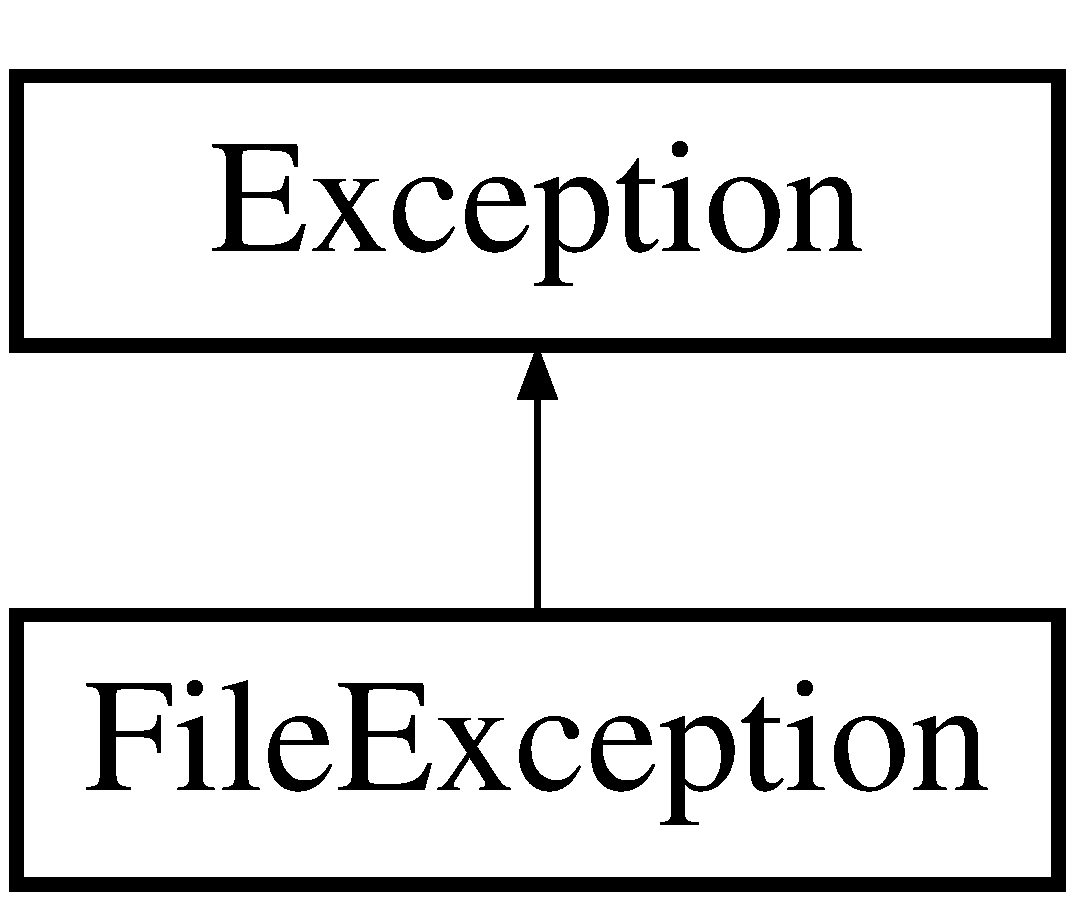
\includegraphics[height=2.000000cm]{class_simple_lion_1_1_file_exception}
\end{center}
\end{figure}
\subsection*{Public Member Functions}
\begin{DoxyCompactItemize}
\item 
\hyperlink{class_simple_lion_1_1_file_exception_a87f2f2594d5a2732de3559816137cccb}{\-\_\-\-\_\-construct} (\$filepath, \$msg)
\item 
\hyperlink{class_simple_lion_1_1_file_exception_a7516ca30af0db3cdbf9a7739b48ce91d}{\-\_\-\-\_\-to\-String} ()
\end{DoxyCompactItemize}


\subsection{Detailed Description}
An exception to be thrown on file error. 

\subsection{Constructor \& Destructor Documentation}
\hypertarget{class_simple_lion_1_1_file_exception_a87f2f2594d5a2732de3559816137cccb}{\index{Simple\-Lion\-::\-File\-Exception@{Simple\-Lion\-::\-File\-Exception}!\-\_\-\-\_\-construct@{\-\_\-\-\_\-construct}}
\index{\-\_\-\-\_\-construct@{\-\_\-\-\_\-construct}!SimpleLion::FileException@{Simple\-Lion\-::\-File\-Exception}}
\subsubsection[{\-\_\-\-\_\-construct}]{\setlength{\rightskip}{0pt plus 5cm}\-\_\-\-\_\-construct (
\begin{DoxyParamCaption}
\item[{}]{\$filepath, }
\item[{}]{\$msg}
\end{DoxyParamCaption}
)}}\label{class_simple_lion_1_1_file_exception_a87f2f2594d5a2732de3559816137cccb}
$<$A constructor from file path and error message.

$<$ 
\begin{DoxyParams}{Parameters}
{\em \$filepath} & A path to the file where error occured. \\
\hline
{\em \$msg} & Error message. \\
\hline
\end{DoxyParams}


\subsection{Member Function Documentation}
\hypertarget{class_simple_lion_1_1_file_exception_a7516ca30af0db3cdbf9a7739b48ce91d}{\index{Simple\-Lion\-::\-File\-Exception@{Simple\-Lion\-::\-File\-Exception}!\-\_\-\-\_\-to\-String@{\-\_\-\-\_\-to\-String}}
\index{\-\_\-\-\_\-to\-String@{\-\_\-\-\_\-to\-String}!SimpleLion::FileException@{Simple\-Lion\-::\-File\-Exception}}
\subsubsection[{\-\_\-\-\_\-to\-String}]{\setlength{\rightskip}{0pt plus 5cm}\-\_\-\-\_\-to\-String (
\begin{DoxyParamCaption}
{}
\end{DoxyParamCaption}
)}}\label{class_simple_lion_1_1_file_exception_a7516ca30af0db3cdbf9a7739b48ce91d}
$<$A function that returns error message.

$<$ \begin{DoxyReturn}{Returns}
Error message with file path. 
\end{DoxyReturn}


The documentation for this class was generated from the following file\-:\begin{DoxyCompactItemize}
\item 
\hyperlink{exceptions_8inc_8php}{exceptions.\-inc.\-php}\end{DoxyCompactItemize}

\hypertarget{class_simple_lion_1_1_filesystem_exception}{\section{Filesystem\-Exception Class Reference}
\label{class_simple_lion_1_1_filesystem_exception}\index{Filesystem\-Exception@{Filesystem\-Exception}}
}


An exception to be thrown on directory error.  


Inheritance diagram for Filesystem\-Exception\-:\begin{figure}[H]
\begin{center}
\leavevmode
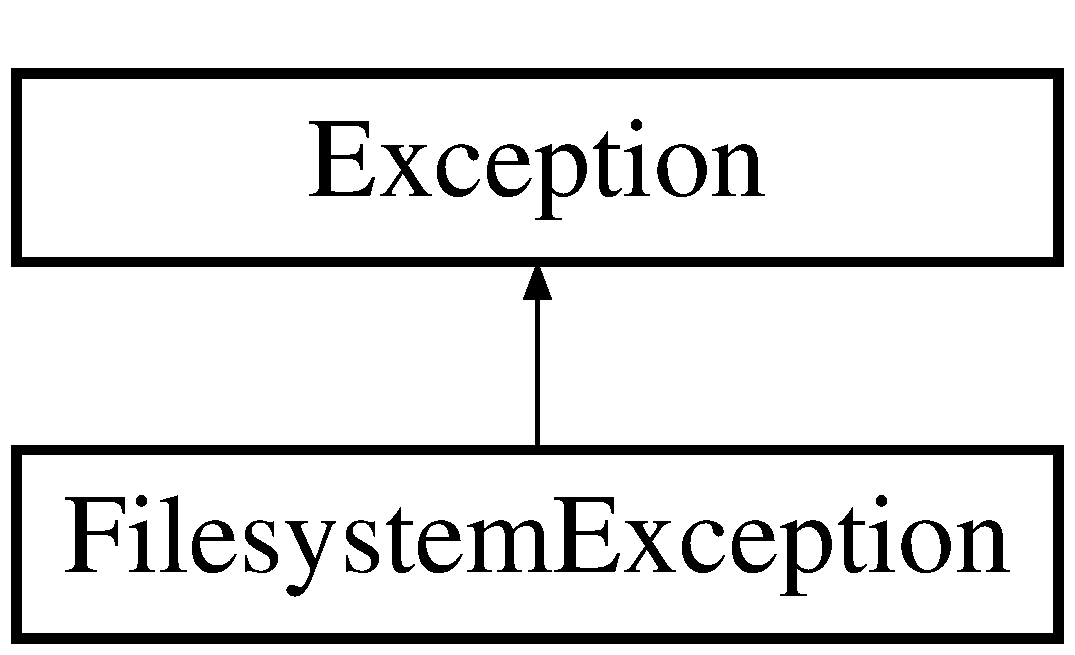
\includegraphics[height=2.000000cm]{class_simple_lion_1_1_filesystem_exception}
\end{center}
\end{figure}
\subsection*{Public Member Functions}
\begin{DoxyCompactItemize}
\item 
\hyperlink{class_simple_lion_1_1_filesystem_exception_a721bfc707580bfe92e1da7bc2a5be13c}{\-\_\-\-\_\-construct} (\$dirpath, \$msg)
\item 
\hyperlink{class_simple_lion_1_1_filesystem_exception_a7516ca30af0db3cdbf9a7739b48ce91d}{\-\_\-\-\_\-to\-String} ()
\end{DoxyCompactItemize}


\subsection{Detailed Description}
An exception to be thrown on directory error. 

\subsection{Constructor \& Destructor Documentation}
\hypertarget{class_simple_lion_1_1_filesystem_exception_a721bfc707580bfe92e1da7bc2a5be13c}{\index{Simple\-Lion\-::\-Filesystem\-Exception@{Simple\-Lion\-::\-Filesystem\-Exception}!\-\_\-\-\_\-construct@{\-\_\-\-\_\-construct}}
\index{\-\_\-\-\_\-construct@{\-\_\-\-\_\-construct}!SimpleLion::FilesystemException@{Simple\-Lion\-::\-Filesystem\-Exception}}
\subsubsection[{\-\_\-\-\_\-construct}]{\setlength{\rightskip}{0pt plus 5cm}\-\_\-\-\_\-construct (
\begin{DoxyParamCaption}
\item[{}]{\$dirpath, }
\item[{}]{\$msg}
\end{DoxyParamCaption}
)}}\label{class_simple_lion_1_1_filesystem_exception_a721bfc707580bfe92e1da7bc2a5be13c}
$<$A constructor from path and error message.

$<$ 
\begin{DoxyParams}{Parameters}
{\em \$dirpath} & A path to where error occured. \\
\hline
{\em \$msg} & Error message. \\
\hline
\end{DoxyParams}


\subsection{Member Function Documentation}
\hypertarget{class_simple_lion_1_1_filesystem_exception_a7516ca30af0db3cdbf9a7739b48ce91d}{\index{Simple\-Lion\-::\-Filesystem\-Exception@{Simple\-Lion\-::\-Filesystem\-Exception}!\-\_\-\-\_\-to\-String@{\-\_\-\-\_\-to\-String}}
\index{\-\_\-\-\_\-to\-String@{\-\_\-\-\_\-to\-String}!SimpleLion::FilesystemException@{Simple\-Lion\-::\-Filesystem\-Exception}}
\subsubsection[{\-\_\-\-\_\-to\-String}]{\setlength{\rightskip}{0pt plus 5cm}\-\_\-\-\_\-to\-String (
\begin{DoxyParamCaption}
{}
\end{DoxyParamCaption}
)}}\label{class_simple_lion_1_1_filesystem_exception_a7516ca30af0db3cdbf9a7739b48ce91d}
$<$A function that returns error message.

$<$ \begin{DoxyReturn}{Returns}
Error message with path. 
\end{DoxyReturn}


The documentation for this class was generated from the following file\-:\begin{DoxyCompactItemize}
\item 
\hyperlink{exceptions_8inc_8php}{exceptions.\-inc.\-php}\end{DoxyCompactItemize}

\hypertarget{class_simple_lion_1_1_localization}{\section{Localization Class Reference}
\label{class_simple_lion_1_1_localization}\index{Localization@{Localization}}
}


A class representing the \hyperlink{class_simple_lion_1_1_localization}{Localization} engine.  


\subsection*{Public Member Functions}
\begin{DoxyCompactItemize}
\item 
\hyperlink{class_simple_lion_1_1_localization_aff9c6ae8a009c4a2c42523c416af6f21}{\-\_\-\-\_\-construct} (\$path, \$locale=null)
\item 
\hyperlink{class_simple_lion_1_1_localization_a1bef7c51e9f6a97840f016a8f0a615ae}{set\-Locale} (\$locale)
\item 
\hyperlink{class_simple_lion_1_1_localization_abb5a777a3f4217d9473883e80cae4b53}{query} (\$query\-String)
\item 
\hyperlink{class_simple_lion_1_1_localization_a357800ef35be75a58766fdb86090211b}{locale\-List} ()
\item 
\hyperlink{class_simple_lion_1_1_localization_a129b22867863a1b34ffd83448a8546bd}{to\-S\-L\-L\-F} ()
\end{DoxyCompactItemize}


\subsection{Detailed Description}
A class representing the \hyperlink{class_simple_lion_1_1_localization}{Localization} engine. 

\subsection{Constructor \& Destructor Documentation}
\hypertarget{class_simple_lion_1_1_localization_aff9c6ae8a009c4a2c42523c416af6f21}{\index{Simple\-Lion\-::\-Localization@{Simple\-Lion\-::\-Localization}!\-\_\-\-\_\-construct@{\-\_\-\-\_\-construct}}
\index{\-\_\-\-\_\-construct@{\-\_\-\-\_\-construct}!SimpleLion::Localization@{Simple\-Lion\-::\-Localization}}
\subsubsection[{\-\_\-\-\_\-construct}]{\setlength{\rightskip}{0pt plus 5cm}\-\_\-\-\_\-construct (
\begin{DoxyParamCaption}
\item[{}]{\$path, }
\item[{}]{\$locale = {\ttfamily null}}
\end{DoxyParamCaption}
)}}\label{class_simple_lion_1_1_localization_aff9c6ae8a009c4a2c42523c416af6f21}
$<$A constructor that checks given path for locales, loads locale list and optionally opens and parses the specified locale. Throws \hyperlink{class_simple_lion_1_1_file_exception}{File\-Exception} and \hyperlink{class_simple_lion_1_1_filesystem_exception}{Filesystem\-Exception} on errors.

$<$ 
\begin{DoxyParams}{Parameters}
{\em \$path} & A path to locales. \\
\hline
{\em \$locale} & Optional locale to open and parse. Can be null. \\
\hline
\end{DoxyParams}


\subsection{Member Function Documentation}
\hypertarget{class_simple_lion_1_1_localization_a357800ef35be75a58766fdb86090211b}{\index{Simple\-Lion\-::\-Localization@{Simple\-Lion\-::\-Localization}!locale\-List@{locale\-List}}
\index{locale\-List@{locale\-List}!SimpleLion::Localization@{Simple\-Lion\-::\-Localization}}
\subsubsection[{locale\-List}]{\setlength{\rightskip}{0pt plus 5cm}locale\-List (
\begin{DoxyParamCaption}
{}
\end{DoxyParamCaption}
)}}\label{class_simple_lion_1_1_localization_a357800ef35be75a58766fdb86090211b}
$<$A method that refreshes and returns list of currently available locales.

$<$ \begin{DoxyReturn}{Returns}
Array of currently available locale codes. 
\end{DoxyReturn}
\hypertarget{class_simple_lion_1_1_localization_abb5a777a3f4217d9473883e80cae4b53}{\index{Simple\-Lion\-::\-Localization@{Simple\-Lion\-::\-Localization}!query@{query}}
\index{query@{query}!SimpleLion::Localization@{Simple\-Lion\-::\-Localization}}
\subsubsection[{query}]{\setlength{\rightskip}{0pt plus 5cm}query (
\begin{DoxyParamCaption}
\item[{}]{\$query\-String}
\end{DoxyParamCaption}
)}}\label{class_simple_lion_1_1_localization_abb5a777a3f4217d9473883e80cae4b53}
$<$A method that returns localized string value according to query\-String or error message (to fit in the bad translation' s place).

$<$ 
\begin{DoxyParams}{Parameters}
{\em query\-String} & A query string, formatted this way\-: string\-\_\-name or category\-\_\-name.\-category\-\_\-name.(...).string\-\_\-name \\
\hline
\end{DoxyParams}
\begin{DoxyReturn}{Returns}
Localized string value or error as string. 
\end{DoxyReturn}
\hypertarget{class_simple_lion_1_1_localization_a1bef7c51e9f6a97840f016a8f0a615ae}{\index{Simple\-Lion\-::\-Localization@{Simple\-Lion\-::\-Localization}!set\-Locale@{set\-Locale}}
\index{set\-Locale@{set\-Locale}!SimpleLion::Localization@{Simple\-Lion\-::\-Localization}}
\subsubsection[{set\-Locale}]{\setlength{\rightskip}{0pt plus 5cm}set\-Locale (
\begin{DoxyParamCaption}
\item[{}]{\$locale}
\end{DoxyParamCaption}
)}}\label{class_simple_lion_1_1_localization_a1bef7c51e9f6a97840f016a8f0a615ae}
$<$A method that opens and parsers the specified locale. Throws \hyperlink{class_simple_lion_1_1_file_exception}{File\-Exception} and \hyperlink{class_simple_lion_1_1_filesystem_exception}{Filesystem\-Exception} on errors.

$<$ 
\begin{DoxyParams}{Parameters}
{\em \$locale} & Locale to open and parse. \\
\hline
\end{DoxyParams}
\hypertarget{class_simple_lion_1_1_localization_a129b22867863a1b34ffd83448a8546bd}{\index{Simple\-Lion\-::\-Localization@{Simple\-Lion\-::\-Localization}!to\-S\-L\-L\-F@{to\-S\-L\-L\-F}}
\index{to\-S\-L\-L\-F@{to\-S\-L\-L\-F}!SimpleLion::Localization@{Simple\-Lion\-::\-Localization}}
\subsubsection[{to\-S\-L\-L\-F}]{\setlength{\rightskip}{0pt plus 5cm}to\-S\-L\-L\-F (
\begin{DoxyParamCaption}
{}
\end{DoxyParamCaption}
)}}\label{class_simple_lion_1_1_localization_a129b22867863a1b34ffd83448a8546bd}
$<$A method that returns the \hyperlink{class_simple_lion_1_1_localization}{Localization} object in S\-L\-L\-F format.

$<$ \begin{DoxyReturn}{Returns}
\hyperlink{class_simple_lion_1_1_localization}{Localization} object in S\-L\-L\-F format, as string. 
\end{DoxyReturn}


The documentation for this class was generated from the following file\-:\begin{DoxyCompactItemize}
\item 
\hyperlink{localization_8inc_8php}{localization.\-inc.\-php}\end{DoxyCompactItemize}

\hypertarget{class_simple_lion_1_1_localization_category}{\section{Localization\-Category Class Reference}
\label{class_simple_lion_1_1_localization_category}\index{Localization\-Category@{Localization\-Category}}
}


A class that represents category grouping localization strings.  


\subsection*{Public Member Functions}
\begin{DoxyCompactItemize}
\item 
\hyperlink{class_simple_lion_1_1_localization_category_aa7843dae8184afc5ab27814533e12ba8}{\-\_\-\-\_\-construct} (\$\hyperlink{class_simple_lion_1_1_localization_category_a4b516aaa5fa38da4fed24ab6001627e2}{name}=null)
\item 
\hyperlink{class_simple_lion_1_1_localization_category_abb9f0d6adf1eb9b3b55712056861a247}{valid} ()
\item 
\hyperlink{class_simple_lion_1_1_localization_category_a088bc0c650ebd5e60ba88b9edb572ae0}{add\-Localization\-Entry} (\$entry)
\item 
\hyperlink{class_simple_lion_1_1_localization_category_aec06c962021b0422399570806aa60b69}{get\-Next\-Localization\-Entry} ()
\item 
\hyperlink{class_simple_lion_1_1_localization_category_a32a9975a699b2a415f251389c851c82a}{get\-Localization\-Entry\-At} (\$idx)
\item 
\hyperlink{class_simple_lion_1_1_localization_category_a4e001554d3486c0ed72c5fd912541724}{remove\-Localization\-Entry} (\$idx)
\item 
\hyperlink{class_simple_lion_1_1_localization_category_a0897c03f1447505b6b1c9251c90c6ac3}{get\-Localization\-Entry\-By\-Name} (\$\hyperlink{class_simple_lion_1_1_localization_category_a4b516aaa5fa38da4fed24ab6001627e2}{name})
\item 
\hyperlink{class_simple_lion_1_1_localization_category_a2e8695b4ef92eb532964f98a6957594f}{remove\-Localization\-Entry\-By\-Name} (\$\hyperlink{class_simple_lion_1_1_localization_category_a4b516aaa5fa38da4fed24ab6001627e2}{name})
\item 
\hyperlink{class_simple_lion_1_1_localization_category_a4b516aaa5fa38da4fed24ab6001627e2}{name} ()
\item 
\hyperlink{class_simple_lion_1_1_localization_category_aedfa75bca162c2d66098e1fac13224eb}{reset\-Localization\-Entry\-Iterator} ()
\item 
\hyperlink{class_simple_lion_1_1_localization_category_a9d13e88319d0c8d8802e3fb839fddf13}{localization\-Entries\-At\-End} ()
\item 
\hyperlink{class_simple_lion_1_1_localization_category_a2fe666694997d047711d7653eca2f132}{set\-Name} (\$\hyperlink{class_simple_lion_1_1_localization_category_a4b516aaa5fa38da4fed24ab6001627e2}{name})
\item 
\hyperlink{class_simple_lion_1_1_localization_category_a129b22867863a1b34ffd83448a8546bd}{to\-S\-L\-L\-F} ()
\end{DoxyCompactItemize}


\subsection{Detailed Description}
A class that represents category grouping localization strings. 

\subsection{Constructor \& Destructor Documentation}
\hypertarget{class_simple_lion_1_1_localization_category_aa7843dae8184afc5ab27814533e12ba8}{\index{Simple\-Lion\-::\-Localization\-Category@{Simple\-Lion\-::\-Localization\-Category}!\-\_\-\-\_\-construct@{\-\_\-\-\_\-construct}}
\index{\-\_\-\-\_\-construct@{\-\_\-\-\_\-construct}!SimpleLion::LocalizationCategory@{Simple\-Lion\-::\-Localization\-Category}}
\subsubsection[{\-\_\-\-\_\-construct}]{\setlength{\rightskip}{0pt plus 5cm}\-\_\-\-\_\-construct (
\begin{DoxyParamCaption}
\item[{}]{\$name = {\ttfamily null}}
\end{DoxyParamCaption}
)}}\label{class_simple_lion_1_1_localization_category_aa7843dae8184afc5ab27814533e12ba8}
$<$A constructor from name.

$<$ 
\begin{DoxyParams}{Parameters}
{\em \$name} & Name of the category, can be null but then the category will be invalid. \\
\hline
\end{DoxyParams}


\subsection{Member Function Documentation}
\hypertarget{class_simple_lion_1_1_localization_category_a088bc0c650ebd5e60ba88b9edb572ae0}{\index{Simple\-Lion\-::\-Localization\-Category@{Simple\-Lion\-::\-Localization\-Category}!add\-Localization\-Entry@{add\-Localization\-Entry}}
\index{add\-Localization\-Entry@{add\-Localization\-Entry}!SimpleLion::LocalizationCategory@{Simple\-Lion\-::\-Localization\-Category}}
\subsubsection[{add\-Localization\-Entry}]{\setlength{\rightskip}{0pt plus 5cm}add\-Localization\-Entry (
\begin{DoxyParamCaption}
\item[{}]{\$entry}
\end{DoxyParamCaption}
)}}\label{class_simple_lion_1_1_localization_category_a088bc0c650ebd5e60ba88b9edb572ae0}
$<$A function that adds a string or category into the category object.

$<$ 
\begin{DoxyParams}{Parameters}
{\em \$entry} & A string or category to insert into the category object. \\
\hline
\end{DoxyParams}
\begin{DoxyReturn}{Returns}
True if the object was inserted, false otherwise. 
\end{DoxyReturn}
\hypertarget{class_simple_lion_1_1_localization_category_a32a9975a699b2a415f251389c851c82a}{\index{Simple\-Lion\-::\-Localization\-Category@{Simple\-Lion\-::\-Localization\-Category}!get\-Localization\-Entry\-At@{get\-Localization\-Entry\-At}}
\index{get\-Localization\-Entry\-At@{get\-Localization\-Entry\-At}!SimpleLion::LocalizationCategory@{Simple\-Lion\-::\-Localization\-Category}}
\subsubsection[{get\-Localization\-Entry\-At}]{\setlength{\rightskip}{0pt plus 5cm}get\-Localization\-Entry\-At (
\begin{DoxyParamCaption}
\item[{}]{\$idx}
\end{DoxyParamCaption}
)}}\label{class_simple_lion_1_1_localization_category_a32a9975a699b2a415f251389c851c82a}
$<$A function that returns string or subcategory from specific index in the subentries array.

$<$ 
\begin{DoxyParams}{Parameters}
{\em \$idx} & Index of the entry. \\
\hline
\end{DoxyParams}
\begin{DoxyReturn}{Returns}
Specified entry or null. 
\end{DoxyReturn}
\hypertarget{class_simple_lion_1_1_localization_category_a0897c03f1447505b6b1c9251c90c6ac3}{\index{Simple\-Lion\-::\-Localization\-Category@{Simple\-Lion\-::\-Localization\-Category}!get\-Localization\-Entry\-By\-Name@{get\-Localization\-Entry\-By\-Name}}
\index{get\-Localization\-Entry\-By\-Name@{get\-Localization\-Entry\-By\-Name}!SimpleLion::LocalizationCategory@{Simple\-Lion\-::\-Localization\-Category}}
\subsubsection[{get\-Localization\-Entry\-By\-Name}]{\setlength{\rightskip}{0pt plus 5cm}get\-Localization\-Entry\-By\-Name (
\begin{DoxyParamCaption}
\item[{}]{\$name}
\end{DoxyParamCaption}
)}}\label{class_simple_lion_1_1_localization_category_a0897c03f1447505b6b1c9251c90c6ac3}
$<$A function that returns string or subcategory with specific name..

$<$ 
\begin{DoxyParams}{Parameters}
{\em \$name} & Name of the entry. \\
\hline
\end{DoxyParams}
\begin{DoxyReturn}{Returns}
Specified entry or null. 
\end{DoxyReturn}
\hypertarget{class_simple_lion_1_1_localization_category_aec06c962021b0422399570806aa60b69}{\index{Simple\-Lion\-::\-Localization\-Category@{Simple\-Lion\-::\-Localization\-Category}!get\-Next\-Localization\-Entry@{get\-Next\-Localization\-Entry}}
\index{get\-Next\-Localization\-Entry@{get\-Next\-Localization\-Entry}!SimpleLion::LocalizationCategory@{Simple\-Lion\-::\-Localization\-Category}}
\subsubsection[{get\-Next\-Localization\-Entry}]{\setlength{\rightskip}{0pt plus 5cm}get\-Next\-Localization\-Entry (
\begin{DoxyParamCaption}
{}
\end{DoxyParamCaption}
)}}\label{class_simple_lion_1_1_localization_category_aec06c962021b0422399570806aa60b69}
$<$A function that returns next string or subcategory from category object.

$<$ \begin{DoxyReturn}{Returns}
Next string or subcategory from category object or null if reached end of the arrray. 
\end{DoxyReturn}
\hypertarget{class_simple_lion_1_1_localization_category_a9d13e88319d0c8d8802e3fb839fddf13}{\index{Simple\-Lion\-::\-Localization\-Category@{Simple\-Lion\-::\-Localization\-Category}!localization\-Entries\-At\-End@{localization\-Entries\-At\-End}}
\index{localization\-Entries\-At\-End@{localization\-Entries\-At\-End}!SimpleLion::LocalizationCategory@{Simple\-Lion\-::\-Localization\-Category}}
\subsubsection[{localization\-Entries\-At\-End}]{\setlength{\rightskip}{0pt plus 5cm}localization\-Entries\-At\-End (
\begin{DoxyParamCaption}
{}
\end{DoxyParamCaption}
)}}\label{class_simple_lion_1_1_localization_category_a9d13e88319d0c8d8802e3fb839fddf13}
$<$A function that returns if the iterator of the subentries array has reached its end.

$<$ \begin{DoxyReturn}{Returns}
True if the iterator of the subentries array has reached its end, false otherwise. 
\end{DoxyReturn}
\hypertarget{class_simple_lion_1_1_localization_category_a4b516aaa5fa38da4fed24ab6001627e2}{\index{Simple\-Lion\-::\-Localization\-Category@{Simple\-Lion\-::\-Localization\-Category}!name@{name}}
\index{name@{name}!SimpleLion::LocalizationCategory@{Simple\-Lion\-::\-Localization\-Category}}
\subsubsection[{name}]{\setlength{\rightskip}{0pt plus 5cm}name (
\begin{DoxyParamCaption}
{}
\end{DoxyParamCaption}
)}}\label{class_simple_lion_1_1_localization_category_a4b516aaa5fa38da4fed24ab6001627e2}
$<$A function that returns name of the category.

$<$ \begin{DoxyReturn}{Returns}
Name of the category or null if the category is not valid. 
\end{DoxyReturn}
\hypertarget{class_simple_lion_1_1_localization_category_a4e001554d3486c0ed72c5fd912541724}{\index{Simple\-Lion\-::\-Localization\-Category@{Simple\-Lion\-::\-Localization\-Category}!remove\-Localization\-Entry@{remove\-Localization\-Entry}}
\index{remove\-Localization\-Entry@{remove\-Localization\-Entry}!SimpleLion::LocalizationCategory@{Simple\-Lion\-::\-Localization\-Category}}
\subsubsection[{remove\-Localization\-Entry}]{\setlength{\rightskip}{0pt plus 5cm}remove\-Localization\-Entry (
\begin{DoxyParamCaption}
\item[{}]{\$idx}
\end{DoxyParamCaption}
)}}\label{class_simple_lion_1_1_localization_category_a4e001554d3486c0ed72c5fd912541724}
$<$A function that removes a string or subcategory from specific index in the subentries array.

$<$ 
\begin{DoxyParams}{Parameters}
{\em \$idx} & Index of the entry. \\
\hline
\end{DoxyParams}
\begin{DoxyReturn}{Returns}
True if the entry was removed, false otherwise. 
\end{DoxyReturn}
\hypertarget{class_simple_lion_1_1_localization_category_a2e8695b4ef92eb532964f98a6957594f}{\index{Simple\-Lion\-::\-Localization\-Category@{Simple\-Lion\-::\-Localization\-Category}!remove\-Localization\-Entry\-By\-Name@{remove\-Localization\-Entry\-By\-Name}}
\index{remove\-Localization\-Entry\-By\-Name@{remove\-Localization\-Entry\-By\-Name}!SimpleLion::LocalizationCategory@{Simple\-Lion\-::\-Localization\-Category}}
\subsubsection[{remove\-Localization\-Entry\-By\-Name}]{\setlength{\rightskip}{0pt plus 5cm}remove\-Localization\-Entry\-By\-Name (
\begin{DoxyParamCaption}
\item[{}]{\$name}
\end{DoxyParamCaption}
)}}\label{class_simple_lion_1_1_localization_category_a2e8695b4ef92eb532964f98a6957594f}
$<$A function that removes string or subcategory with specific name..

$<$ 
\begin{DoxyParams}{Parameters}
{\em \$name} & Name of the entry. \\
\hline
\end{DoxyParams}
\begin{DoxyReturn}{Returns}
True if the entry was removed, false otherwise. 
\end{DoxyReturn}
\hypertarget{class_simple_lion_1_1_localization_category_aedfa75bca162c2d66098e1fac13224eb}{\index{Simple\-Lion\-::\-Localization\-Category@{Simple\-Lion\-::\-Localization\-Category}!reset\-Localization\-Entry\-Iterator@{reset\-Localization\-Entry\-Iterator}}
\index{reset\-Localization\-Entry\-Iterator@{reset\-Localization\-Entry\-Iterator}!SimpleLion::LocalizationCategory@{Simple\-Lion\-::\-Localization\-Category}}
\subsubsection[{reset\-Localization\-Entry\-Iterator}]{\setlength{\rightskip}{0pt plus 5cm}reset\-Localization\-Entry\-Iterator (
\begin{DoxyParamCaption}
{}
\end{DoxyParamCaption}
)}}\label{class_simple_lion_1_1_localization_category_aedfa75bca162c2d66098e1fac13224eb}
$<$ A function, that resets iterator of the subentries array. \hypertarget{class_simple_lion_1_1_localization_category_a2fe666694997d047711d7653eca2f132}{\index{Simple\-Lion\-::\-Localization\-Category@{Simple\-Lion\-::\-Localization\-Category}!set\-Name@{set\-Name}}
\index{set\-Name@{set\-Name}!SimpleLion::LocalizationCategory@{Simple\-Lion\-::\-Localization\-Category}}
\subsubsection[{set\-Name}]{\setlength{\rightskip}{0pt plus 5cm}set\-Name (
\begin{DoxyParamCaption}
\item[{}]{\$name}
\end{DoxyParamCaption}
)}}\label{class_simple_lion_1_1_localization_category_a2fe666694997d047711d7653eca2f132}
$<$A function that sets name of the category.

$<$ 
\begin{DoxyParams}{Parameters}
{\em \$name} & New name of the category. \\
\hline
\end{DoxyParams}
\hypertarget{class_simple_lion_1_1_localization_category_a129b22867863a1b34ffd83448a8546bd}{\index{Simple\-Lion\-::\-Localization\-Category@{Simple\-Lion\-::\-Localization\-Category}!to\-S\-L\-L\-F@{to\-S\-L\-L\-F}}
\index{to\-S\-L\-L\-F@{to\-S\-L\-L\-F}!SimpleLion::LocalizationCategory@{Simple\-Lion\-::\-Localization\-Category}}
\subsubsection[{to\-S\-L\-L\-F}]{\setlength{\rightskip}{0pt plus 5cm}to\-S\-L\-L\-F (
\begin{DoxyParamCaption}
{}
\end{DoxyParamCaption}
)}}\label{class_simple_lion_1_1_localization_category_a129b22867863a1b34ffd83448a8546bd}
$<$A function that returns a category object in S\-L\-L\-F format.

$<$ \begin{DoxyReturn}{Returns}
S\-L\-L\-F representation of the object or null if object is not valid. 
\end{DoxyReturn}
\hypertarget{class_simple_lion_1_1_localization_category_abb9f0d6adf1eb9b3b55712056861a247}{\index{Simple\-Lion\-::\-Localization\-Category@{Simple\-Lion\-::\-Localization\-Category}!valid@{valid}}
\index{valid@{valid}!SimpleLion::LocalizationCategory@{Simple\-Lion\-::\-Localization\-Category}}
\subsubsection[{valid}]{\setlength{\rightskip}{0pt plus 5cm}valid (
\begin{DoxyParamCaption}
{}
\end{DoxyParamCaption}
)}}\label{class_simple_lion_1_1_localization_category_abb9f0d6adf1eb9b3b55712056861a247}
$<$A function that returns if the category object is valid.

$<$ \begin{DoxyReturn}{Returns}
True if the category object is valid -\/ its name must be non-\/empty -\/ and false otherwise. 
\end{DoxyReturn}


The documentation for this class was generated from the following file\-:\begin{DoxyCompactItemize}
\item 
\hyperlink{localization__category_8inc_8php}{localization\-\_\-category.\-inc.\-php}\end{DoxyCompactItemize}

\hypertarget{class_simple_lion_1_1_localization_string}{\section{Localization\-String Class Reference}
\label{class_simple_lion_1_1_localization_string}\index{Localization\-String@{Localization\-String}}
}


A class representing a localized string.  


\subsection*{Public Member Functions}
\begin{DoxyCompactItemize}
\item 
\hyperlink{class_simple_lion_1_1_localization_string_a0a78b62dd316bf5e63a3f5a5f43092b3}{\-\_\-\-\_\-construct} (\$\hyperlink{class_simple_lion_1_1_localization_string_a4b516aaa5fa38da4fed24ab6001627e2}{name}=null, \$\hyperlink{class_simple_lion_1_1_localization_string_aefbfa229f1c9e1fc967bff724a010f9e}{value}=null)
\item 
\hyperlink{class_simple_lion_1_1_localization_string_abb9f0d6adf1eb9b3b55712056861a247}{valid} ()
\item 
\hyperlink{class_simple_lion_1_1_localization_string_a4b516aaa5fa38da4fed24ab6001627e2}{name} ()
\item 
\hyperlink{class_simple_lion_1_1_localization_string_aefbfa229f1c9e1fc967bff724a010f9e}{value} ()
\item 
\hyperlink{class_simple_lion_1_1_localization_string_a2fe666694997d047711d7653eca2f132}{set\-Name} (\$\hyperlink{class_simple_lion_1_1_localization_string_a4b516aaa5fa38da4fed24ab6001627e2}{name})
\item 
\hyperlink{class_simple_lion_1_1_localization_string_a7494441b6ed08a391704971873f31432}{set\-Value} (\$\hyperlink{class_simple_lion_1_1_localization_string_aefbfa229f1c9e1fc967bff724a010f9e}{value})
\item 
\hyperlink{class_simple_lion_1_1_localization_string_a129b22867863a1b34ffd83448a8546bd}{to\-S\-L\-L\-F} ()
\end{DoxyCompactItemize}


\subsection{Detailed Description}
A class representing a localized string. 

\subsection{Constructor \& Destructor Documentation}
\hypertarget{class_simple_lion_1_1_localization_string_a0a78b62dd316bf5e63a3f5a5f43092b3}{\index{Simple\-Lion\-::\-Localization\-String@{Simple\-Lion\-::\-Localization\-String}!\-\_\-\-\_\-construct@{\-\_\-\-\_\-construct}}
\index{\-\_\-\-\_\-construct@{\-\_\-\-\_\-construct}!SimpleLion::LocalizationString@{Simple\-Lion\-::\-Localization\-String}}
\subsubsection[{\-\_\-\-\_\-construct}]{\setlength{\rightskip}{0pt plus 5cm}\-\_\-\-\_\-construct (
\begin{DoxyParamCaption}
\item[{}]{\$name = {\ttfamily null}, }
\item[{}]{\$value = {\ttfamily null}}
\end{DoxyParamCaption}
)}}\label{class_simple_lion_1_1_localization_string_a0a78b62dd316bf5e63a3f5a5f43092b3}
$<$A constructor with parameters.

$<$ 
\begin{DoxyParams}{Parameters}
{\em \$name} & A name identifying the string, null by default. \\
\hline
{\em \$value} & A localized value of the string, null by default. \\
\hline
\end{DoxyParams}


\subsection{Member Function Documentation}
\hypertarget{class_simple_lion_1_1_localization_string_a4b516aaa5fa38da4fed24ab6001627e2}{\index{Simple\-Lion\-::\-Localization\-String@{Simple\-Lion\-::\-Localization\-String}!name@{name}}
\index{name@{name}!SimpleLion::LocalizationString@{Simple\-Lion\-::\-Localization\-String}}
\subsubsection[{name}]{\setlength{\rightskip}{0pt plus 5cm}name (
\begin{DoxyParamCaption}
{}
\end{DoxyParamCaption}
)}}\label{class_simple_lion_1_1_localization_string_a4b516aaa5fa38da4fed24ab6001627e2}
$<$A function returning name identifying the string.

$<$ \begin{DoxyReturn}{Returns}
Name identifying the string. 
\end{DoxyReturn}
\hypertarget{class_simple_lion_1_1_localization_string_a2fe666694997d047711d7653eca2f132}{\index{Simple\-Lion\-::\-Localization\-String@{Simple\-Lion\-::\-Localization\-String}!set\-Name@{set\-Name}}
\index{set\-Name@{set\-Name}!SimpleLion::LocalizationString@{Simple\-Lion\-::\-Localization\-String}}
\subsubsection[{set\-Name}]{\setlength{\rightskip}{0pt plus 5cm}set\-Name (
\begin{DoxyParamCaption}
\item[{}]{\$name}
\end{DoxyParamCaption}
)}}\label{class_simple_lion_1_1_localization_string_a2fe666694997d047711d7653eca2f132}
$<$A function that sets name identifying the string.

$<$ 
\begin{DoxyParams}{Parameters}
{\em \$name} & Name identifying the string. \\
\hline
\end{DoxyParams}
\hypertarget{class_simple_lion_1_1_localization_string_a7494441b6ed08a391704971873f31432}{\index{Simple\-Lion\-::\-Localization\-String@{Simple\-Lion\-::\-Localization\-String}!set\-Value@{set\-Value}}
\index{set\-Value@{set\-Value}!SimpleLion::LocalizationString@{Simple\-Lion\-::\-Localization\-String}}
\subsubsection[{set\-Value}]{\setlength{\rightskip}{0pt plus 5cm}set\-Value (
\begin{DoxyParamCaption}
\item[{}]{\$value}
\end{DoxyParamCaption}
)}}\label{class_simple_lion_1_1_localization_string_a7494441b6ed08a391704971873f31432}
$<$A function that sets localized value of the string.

$<$ 
\begin{DoxyParams}{Parameters}
{\em \$value} & Localized value of the string. \\
\hline
\end{DoxyParams}
\hypertarget{class_simple_lion_1_1_localization_string_a129b22867863a1b34ffd83448a8546bd}{\index{Simple\-Lion\-::\-Localization\-String@{Simple\-Lion\-::\-Localization\-String}!to\-S\-L\-L\-F@{to\-S\-L\-L\-F}}
\index{to\-S\-L\-L\-F@{to\-S\-L\-L\-F}!SimpleLion::LocalizationString@{Simple\-Lion\-::\-Localization\-String}}
\subsubsection[{to\-S\-L\-L\-F}]{\setlength{\rightskip}{0pt plus 5cm}to\-S\-L\-L\-F (
\begin{DoxyParamCaption}
{}
\end{DoxyParamCaption}
)}}\label{class_simple_lion_1_1_localization_string_a129b22867863a1b34ffd83448a8546bd}
$<$A function that returns a \hyperlink{class_simple_lion_1_1_localization_string}{Localization\-String} object in the S\-L\-L\-F format.

$<$ \begin{DoxyReturn}{Returns}
\hyperlink{class_simple_lion_1_1_localization_string}{Localization\-String} representation in the S\-L\-L\-F format or null if the object is not valid. 
\end{DoxyReturn}
\hypertarget{class_simple_lion_1_1_localization_string_abb9f0d6adf1eb9b3b55712056861a247}{\index{Simple\-Lion\-::\-Localization\-String@{Simple\-Lion\-::\-Localization\-String}!valid@{valid}}
\index{valid@{valid}!SimpleLion::LocalizationString@{Simple\-Lion\-::\-Localization\-String}}
\subsubsection[{valid}]{\setlength{\rightskip}{0pt plus 5cm}valid (
\begin{DoxyParamCaption}
{}
\end{DoxyParamCaption}
)}}\label{class_simple_lion_1_1_localization_string_abb9f0d6adf1eb9b3b55712056861a247}
$<$A function returning if this \hyperlink{class_simple_lion_1_1_localization_string}{Localization\-String} object is valid.

$<$ \begin{DoxyReturn}{Returns}
True if the \hyperlink{class_simple_lion_1_1_localization_string}{Localization\-String} is valid, which means it has non-\/empty name and value, false otherwise. 
\end{DoxyReturn}
\hypertarget{class_simple_lion_1_1_localization_string_aefbfa229f1c9e1fc967bff724a010f9e}{\index{Simple\-Lion\-::\-Localization\-String@{Simple\-Lion\-::\-Localization\-String}!value@{value}}
\index{value@{value}!SimpleLion::LocalizationString@{Simple\-Lion\-::\-Localization\-String}}
\subsubsection[{value}]{\setlength{\rightskip}{0pt plus 5cm}value (
\begin{DoxyParamCaption}
{}
\end{DoxyParamCaption}
)}}\label{class_simple_lion_1_1_localization_string_aefbfa229f1c9e1fc967bff724a010f9e}
$<$A function returning localized value of the string.

$<$ \begin{DoxyReturn}{Returns}
Localized value of the string. 
\end{DoxyReturn}


The documentation for this class was generated from the following file\-:\begin{DoxyCompactItemize}
\item 
\hyperlink{localization__string_8inc_8php}{localization\-\_\-string.\-inc.\-php}\end{DoxyCompactItemize}

\chapter{File Documentation}
\hypertarget{exceptions_8inc_8php}{\section{exceptions.\-inc.\-php File Reference}
\label{exceptions_8inc_8php}\index{exceptions.\-inc.\-php@{exceptions.\-inc.\-php}}
}


A part of the \hyperlink{namespace_simple_lion}{Simple\-Lion} project -\/ P\-H\-P module. Exceptions for the module.  


\subsection*{Data Structures}
\begin{DoxyCompactItemize}
\item 
class \hyperlink{class_simple_lion_1_1_file_exception}{File\-Exception}
\begin{DoxyCompactList}\small\item\em An exception to be thrown on file error. \end{DoxyCompactList}\item 
class \hyperlink{class_simple_lion_1_1_filesystem_exception}{Filesystem\-Exception}
\begin{DoxyCompactList}\small\item\em An exception to be thrown on directory error. \end{DoxyCompactList}\end{DoxyCompactItemize}
\subsection*{Namespaces}
\begin{DoxyCompactItemize}
\item 
\hyperlink{namespace_simple_lion}{Simple\-Lion}
\begin{DoxyCompactList}\small\item\em A global namespace for the \hyperlink{namespace_simple_lion}{Simple\-Lion} project -\/ P\-H\-P module. \end{DoxyCompactList}\end{DoxyCompactItemize}


\subsection{Detailed Description}
A part of the \hyperlink{namespace_simple_lion}{Simple\-Lion} project -\/ P\-H\-P module. Exceptions for the module. \begin{DoxyAuthor}{Author}
Phitherek\-\_\- 
\end{DoxyAuthor}
\begin{DoxyDate}{Date}
2013 
\end{DoxyDate}
\begin{DoxyVersion}{Version}
0.\-1 
\end{DoxyVersion}

\hypertarget{localization_8inc_8php}{\section{localization.\-inc.\-php File Reference}
\label{localization_8inc_8php}\index{localization.\-inc.\-php@{localization.\-inc.\-php}}
}


A part of the \hyperlink{namespace_simple_lion}{Simple\-Lion} project -\/ P\-H\-P module. The main class representing a Localization engine.  


\subsection*{Data Structures}
\begin{DoxyCompactItemize}
\item 
class \hyperlink{class_simple_lion_1_1_localization}{Localization}
\begin{DoxyCompactList}\small\item\em A class representing the \hyperlink{class_simple_lion_1_1_localization}{Localization} engine. \end{DoxyCompactList}\end{DoxyCompactItemize}
\subsection*{Namespaces}
\begin{DoxyCompactItemize}
\item 
\hyperlink{namespace_simple_lion}{Simple\-Lion}
\begin{DoxyCompactList}\small\item\em A global namespace for the \hyperlink{namespace_simple_lion}{Simple\-Lion} project -\/ P\-H\-P module. \end{DoxyCompactList}\end{DoxyCompactItemize}


\subsection{Detailed Description}
A part of the \hyperlink{namespace_simple_lion}{Simple\-Lion} project -\/ P\-H\-P module. The main class representing a Localization engine. \begin{DoxyAuthor}{Author}
Phitherek\-\_\- 
\end{DoxyAuthor}
\begin{DoxyDate}{Date}
2013 
\end{DoxyDate}
\begin{DoxyVersion}{Version}
0.\-1 
\end{DoxyVersion}

\hypertarget{localization__category_8inc_8php}{\section{localization\-\_\-category.\-inc.\-php File Reference}
\label{localization__category_8inc_8php}\index{localization\-\_\-category.\-inc.\-php@{localization\-\_\-category.\-inc.\-php}}
}


A part of the \hyperlink{namespace_simple_lion}{Simple\-Lion} project -\/ P\-H\-P module. A class that represents category grouping localization strings.  


\subsection*{Data Structures}
\begin{DoxyCompactItemize}
\item 
class \hyperlink{class_simple_lion_1_1_localization_category}{Localization\-Category}
\begin{DoxyCompactList}\small\item\em A class that represents category grouping localization strings. \end{DoxyCompactList}\end{DoxyCompactItemize}
\subsection*{Namespaces}
\begin{DoxyCompactItemize}
\item 
\hyperlink{namespace_simple_lion}{Simple\-Lion}
\begin{DoxyCompactList}\small\item\em A global namespace for the \hyperlink{namespace_simple_lion}{Simple\-Lion} project -\/ P\-H\-P module. \end{DoxyCompactList}\end{DoxyCompactItemize}


\subsection{Detailed Description}
A part of the \hyperlink{namespace_simple_lion}{Simple\-Lion} project -\/ P\-H\-P module. A class that represents category grouping localization strings. \begin{DoxyAuthor}{Author}
Phitherek\-\_\- 
\end{DoxyAuthor}
\begin{DoxyDate}{Date}
2013 
\end{DoxyDate}
\begin{DoxyVersion}{Version}
0.\-1 
\end{DoxyVersion}

\hypertarget{localization__string_8inc_8php}{\section{localization\-\_\-string.\-inc.\-php File Reference}
\label{localization__string_8inc_8php}\index{localization\-\_\-string.\-inc.\-php@{localization\-\_\-string.\-inc.\-php}}
}


A part of the \hyperlink{namespace_simple_lion}{Simple\-Lion} project -\/ P\-H\-P module. A class representing a localized string.  


\subsection*{Data Structures}
\begin{DoxyCompactItemize}
\item 
class \hyperlink{class_simple_lion_1_1_localization_string}{Localization\-String}
\begin{DoxyCompactList}\small\item\em A class representing a localized string. \end{DoxyCompactList}\end{DoxyCompactItemize}
\subsection*{Namespaces}
\begin{DoxyCompactItemize}
\item 
\hyperlink{namespace_simple_lion}{Simple\-Lion}
\begin{DoxyCompactList}\small\item\em A global namespace for the \hyperlink{namespace_simple_lion}{Simple\-Lion} project -\/ P\-H\-P module. \end{DoxyCompactList}\end{DoxyCompactItemize}


\subsection{Detailed Description}
A part of the \hyperlink{namespace_simple_lion}{Simple\-Lion} project -\/ P\-H\-P module. A class representing a localized string. \begin{DoxyAuthor}{Author}
Phitherek\-\_\- 
\end{DoxyAuthor}
\begin{DoxyDate}{Date}
2013 
\end{DoxyDate}
\begin{DoxyVersion}{Version}
0.\-1 
\end{DoxyVersion}

\hypertarget{simplelion-php_8php}{\section{simplelion-\/php.php File Reference}
\label{simplelion-php_8php}\index{simplelion-\/php.\-php@{simplelion-\/php.\-php}}
}


A global file for inclusion of all the \hyperlink{namespace_simple_lion}{Simple\-Lion} project -\/ P\-H\-P module classes.  




\subsection{Detailed Description}
A global file for inclusion of all the \hyperlink{namespace_simple_lion}{Simple\-Lion} project -\/ P\-H\-P module classes. \begin{DoxyAuthor}{Author}
Phitherek\-\_\- 
\end{DoxyAuthor}
\begin{DoxyDate}{Date}
2013 
\end{DoxyDate}
\begin{DoxyVersion}{Version}
0.\-1 
\end{DoxyVersion}

%--- End generated contents ---

% Index
\newpage
\phantomsection
\addcontentsline{toc}{part}{Index}
\printindex

\end{document}
